% \pdfminorversion=4 
\documentclass[
	usepdftitle=false,
% 	handout,
% 	notes,
% 	fleqn,
	hyperref={
		pdfauthor={Martin Genzel},
		pdftitle={Feature Selection Theory},
		pdfsubject={Workshop},
		pdfcreator={LaTeX},
	}
]{beamer}

%%% Encoding of files
\usepackage[utf8]{inputenc}

%%% Preamble (packages, definitions, settings)
% ------------- Packages

%--------------------------------------------------------------------------------
%---- Julia highlighting settings
%--------------------------------------------------------------------------------
\usepackage{beramono}
\usepackage{listings}

\lstdefinelanguage{julia}{morekeywords={abstract,break,case,catch,const,continue,do,else,elseif,%
      end,export,false,for,function,immutable,import,importall,if,in,%
      macro,module,otherwise,quote,return,switch,true,try,type,typealias,%
      using,while},%
   sensitive=true,%
   morecomment=[l]\#,%
   morecomment=[n]{\#=}{=\#},%
   morestring=[s]{"}{"},%
   morestring=[m]{'}{'},%
}[keywords,comments,strings]%


% \usepackage{default}

%%% Doc: http://mirror.informatik.uni-mannheim.de/pub/mirrors/tex-archive/macros/latex/contrib/xargs/xargs.pdf
% More than one optional argument
\usepackage{xargs}

%%%
% IfThenElse
\usepackage{ifthen}

%%% Doc: ftp://ftp.mpi-sb.mpg.de/pub/tex/mirror/ftp.dante.de/pub/tex/macros/latex/contrib/etoolbox/etoolbox.pdf
% Programming in LaTeX
\usepackage{etoolbox}

%%% Doc: ftp://tug.ctan.org/pub/tex-archive/macros/latex/required/babel/babel.pdf
% Language setting
\usepackage[
%	german,
% 	ngerman,
	english,
%	french,
]{babel}

%%% Doc: ftp://tug.ctan.org/pub/tex-archive/macros/latex/required/graphics/grfguide.pdf
% Graphics
\usepackage[%
	%final,
	%draft % do not include images (faster)
]{graphicx}

\usepackage{array}
\usepackage{multicol}
\usepackage{wrapfig}

% \usepackage{memh­fixc}
% \usepackage{memoir}

\usepackage{relsize}

\usepackage{mdframed}

% \usepackage{enumitem}

%%%
% This package is used to create two-sided presentations with notes
\usepackage{pgfpages}

\usepackage{tikz}
\usetikzlibrary{arrows,shapes,calc}
\newcommand{\tikzmark}[2]{\tikz[overlay,remember picture] \node[minimum width=1.5em] (#1) {#2};}
\newcommand{\tikzcoord}[1]{\tikz[overlay,remember picture] \coordinate (#1);}
\makeatletter
\protected\def\tikz@nonactivecolon{\ifmmode\mathrel{\mathop\ordinarycolon}\else:\fi} 
\makeatother

\newcommand*\circled[1]{\tikz[baseline=(char.base)]{
            \node[shape=circle,draw,inner sep=2pt] (char) {#1};}}


% Put text somewhere on the slide
% \def\Put(#1,#2)#3{\leavevmode\makebox(0,0){\put(#1,#2){#3}}}
\usepackage[absolute,overlay]{textpos}

%%% Doc: ftp://tug.ctan.org/pub/tex-archive/macros/latex/contrib/mh/doc/mathtools.pdf
% Erweitert amsmath und behebt einige Bugs
\usepackage[fixamsmath,disallowspaces]{mathtools}
% Formelnummern nur anzeigen, wenn auch eine Referenz existiert
\mathtoolsset{showonlyrefs}
\mathtoolsset{centercolon=true}
% \usepackage{autonum}

\usepackage{mathrsfs}

\usepackage{bm}

\usepackage{dsfont}
\usepackage{animate}
\usepackage{xcolor}
\usepackage{mdframed}

% ------------- Definitions

%%% Programming
% Falls #2 definiert/nichtleer ist, so schreibe #3, sonst #1
\newcommand{\ifargdef}[3][{}]{\ifthenelse{\equal{#2}{}}{#1}{#3}}

%%% Colors
\definecolor{red}{rgb}{1,0,0}
\definecolor{blue}{rgb}{0,0,1}
\definecolor{green}{rgb}{0.2,0.6,0.15}
\definecolor{darkgreen}{rgb}{0,0.5,0}
\definecolor{lightblue}{rgb}{0,0.5,1}
\definecolor{white}{rgb}{1,1,1}
\definecolor{bluegreen}{rgb}{0,0.5,0.5}
\definecolor{violet}{rgb}{0.5,0,0.5}
\definecolor{ZurichBlue}{rgb}{.35,.35,.73}
\definecolor{TUred}{rgb}{0.7,0,0}
% \definecolor{red}{rgb}{1,0,0}
% \definecolor{blue}{rgb}{0,0,1}
% \definecolor{green}{rgb}{0.2,0.6,0.15}
% \definecolor{darkgreen}{rgb}{0,0.5,0}
% \definecolor{lightblue}{rgb}{0,0.5,1}
% %\definecolor{white}{rgb}{0,0,0}
% \definecolor{bluegreen}{rgb}{0,0.5,0.5}
% \definecolor{violet}{rgb}{0.5,0,0.5}
% \definecolor{ZurichBlue}{rgb}{.35,.35,.73}

\setbeamercolor{highlightbox}{fg=black,bg=ZurichBlue}

% no frame counting in appendix, use together with 'noframenumbering' as frame option
\makeatletter
\preto{\appendix}{%
  \patchcmd{\beamer@continueautobreak}{\refstepcounter{framenumber}}{}{}{}}
\makeatother

% Keep the frame title, if there is a framebreak
\setbeamertemplate{frametitle continuation}{}
% Break frame within a theorem
\newcommand*{\theorembreak}{\usebeamertemplate{theorem end}\framebreak\usebeamertemplate{theorem begin}}
% Definitions highlighting
\newcommand<>{\define}[1]{{\color#2{green} #1}}

\newcommand{\citeref}[1]{{\tiny{\color{gray}#1}}}

\newtheorem{algorithm}{Algorithm}
\newtheorem{proposition}{Proposition}


% ------------- Settings

\mode<presentation>{
	\usetheme{Boadilla}
% 	\useoutertheme{infolines}
% 	\useinnertheme{rounded}
	\usecolortheme{beaver}
	\setbeamercovered{transparent}
	
% Make the default 'red' of beaver darker
	\definecolor{darkred}{rgb}{.65,0,0}
	\setbeamercolor{structure}{fg=ZurichBlue}
	
	\setbeamercolor{block title}{use=structure,fg=white,bg=darkred!80!white}
	\setbeamercolor{block body}{use=structure,fg=black,bg=gray!20!white}
	
	
	\setbeamercolor{frametitle}{bg=gray!20!white}
	
	% Frame title with logo in the right corner
	\setbeamertemplate{frametitle}
	{
		\nointerlineskip
		\begin{beamercolorbox}[sep=0.3cm,wd=\paperwidth]{frametitle}
			\vbox{}\vskip-1ex%
			\strut\insertframetitle\strut \hfill 
			\vskip-1.5ex%
		\end{beamercolorbox}
	}

% 	\setbeamertemplate{footline}[default]
% 	\setbeameroption{show notes on second screen}
% 	\setbeameroption{show notes}
	\setbeamercovered{invisible}
}

\beamertemplatenavigationsymbolsempty

\makeatletter
% add a macro that saves its argument
\newcommand{\footlineextra}[1]{\gdef\insertfootlineextra{#1}}
\newbox\footlineextrabox

% add a beamer template that sets the saved argument in a box.
% The * means that the beamer font and color "footline extra" are automatically added. 
\defbeamertemplate*{footline extra}{default}{
    \begin{beamercolorbox}[ht=2.25ex,dp=1ex,leftskip=\Gm@lmargin]{footline extra}
    \insertfootlineextra
    %\par\vspace{2.5pt}
    \end{beamercolorbox}
}

\addtobeamertemplate{footline}{%
    % set the box with the extra footline material but make it add no vertical space
    \setbox\footlineextrabox=\vbox{\usebeamertemplate*{footline extra}}
    \vskip -\ht\footlineextrabox
    \vskip -\dp\footlineextrabox
    \box\footlineextrabox%
}
{}

% patch \begin{frame} to reset the footline extra material
\let\beamer@original@frame=\frame
\def\frame{\gdef\insertfootlineextra{}\beamer@original@frame}
\footlineextra{}
\makeatother

\newcommand<>{\uncoverubrace}[2]{%
  \onslide#3 \underbrace{ \onslide<1->%
  #1%
  \onslide#3 }_{#2} \onslide<1->%
}

\setbeamertemplate{itemize items}[triangle]

%%% Math macros
%%% Mathematische Makros

%%% Umgebungen

%%% Allgemeines
% flexibler Klammerbefehl, #1=links, #2=rechts, #3=Größe (normal, auto, opauto, \[sizecmd]), #4=Inhalt
\newcommandx{\braces}[4]{%
\ifstrequal{#3}{normal}{#1#4#2}{%
\ifstrequal{#3}{auto}{\left#1#4\right#2}{%
\ifstrequal{#3}{opauto}{\opleft#1#4\opright#2}{%
#3#1#4#3#2}}}%
}
% Klammern für Operatoren (entfernt das Spacing vor und nach der Klammer)
\newcommand{\opleft}[1]{\mathopen{}\left#1}
\newcommand{\opright}[1]{\right#1\mathclose{}}
% Anmerkung über Operatoren
\newcommandx{\opannot}[3][3=\downarrow]{\stackrel{\mathclap{\substack{#1 \\ #3 \vspace{2pt}}}}{#2}}
% Anmerkung vor einer Zeile
\newcommandx{\lineannot}[3][3=\rightarrow]{\mathllap{\boxed{\text{\textsmaller{#1}}} #3} #2}
% Anmerkung vor einer Zeile (mehrzeilig)
\newcommandx{\multilineannot}[4][4=\rightarrow]{\mathllap{\boxed{\parbox{#1}{\RaggedRight\textsmaller{#2}}} #4} #3}
% Anmerkung zwischen zwei Zeilen
\newcommand{\interannot}[1]{\boxed{\text{\textsmaller{#1}}}} 
% Anmerkung zwischen zwei Zeilen (mehrzeilig)
\newcommand{\multiinterannot}[2][.5\textwidth]{\boxed{\parbox{#1}{\RaggedRight\textsmaller{#2}}}} 

%%% Zahlenmengen
\newcommand{\N}{\mathbb{N}} % natürliche Zahlen
\newcommand{\Nzero}{\mathbb{N}_0} % natürliche Zahlen mit Null
\newcommand{\Z}{\mathbb{Z}} % ganze Zahlen
\newcommand{\Q}{\mathbb{Q}} % rationale Zahlen
\newcommand{\R}{\mathbb{R}} % reelle Zahlen
\newcommand{\Rpos}{\mathbb{R}_{>0}} % positive reelle Zahlen
\newcommand{\C}{\mathbb{C}} % komplexe Zahlen
\newcommand{\K}{\mathbb{K}} % reelle oder komplexe Zahlen
%\newcommand{\H}{{H}} % reelle oder komplexe Zahlen

%%% Aussagenlogik
% \renewcommand{\mid}{:} % Trennung der Bedingung bei der Angabe von Mengen
\renewcommand{\iff}{\Leftrightarrow} % genau dann wenn
\renewcommand{\implies}{\Rightarrow} % impliziert
\newcommand{\suchthat}[1][normal]{\ifstrequal{#1}{normal}{\mid}{#1|}}

%%% Mengen und Topologie
\newcommand{\setcompl}[1]{#1^c} % Mengenkomplement
\newcommand{\cardinality}{\#}
\newcommand{\union}{\cup} % Vereinigung
\newcommand{\bigunion}{\bigcup} % Vereinigung
\newcommand{\intersec}{\cap} % Schnittmenge
\newcommand{\bigintersec}{\bigcap} % Schnittmenge
\newcommand{\boundary}[1]{\partial#1} % Rand einer Menge
\newcommand{\clos}[1]{\overline{#1}} % topologischer Abschluss
\newcommand{\interior}[1]{\mathring{#1}} % das innere eine Menge
\newcommand{\dist}[2]{\operatorname{dist}(#1, #2)} % Distanz zwischen zwei Mengen
\newcommandx{\intvcl}[3][1=normal]{\braces{[}{]}{#1}{#2, #3}} % abgeschlossenes Intervall
\newcommandx{\intvop}[3][1=normal]{\braces{(}{)}{#1}{#2, #3}} % offenes Intervall
\newcommandx{\intvclop}[3][1=normal]{\braces{[}{)}{#1}{#2, #3}} % halboffenes Intervall (rechts)
\newcommandx{\intvopcl}[3][1=normal]{\braces{(}{]}{#1}{#2, #3}} % halboffenes Intervall (links)
\newcommand{\indcoeff}[1]{\mathds{1}_{#1}} % Indikatorfunktion für Indizes von Koeffizienten

%%% Analysis
\newcommand{\dotarg}{\ensuremath{\raisebox{.15ex}{$\scriptstyle [\cdot]$}}}
\DeclareMathOperator*{\argmin}{argmin} % argmin
\DeclareMathOperator*{\argmax}{argmax} % argmax
\newcommandx{\abs}[2][1=normal]{\braces{\lvert}{\rvert}{#1}{#2}} % Absolutbetrag
\newcommand{\conj}[1]{\overline{#1}} % komplexe Konjugation
\newcommandx{\ceil}[2][1=normal]{\braces{\lceil}{\rceil}{#1}{#2}} % Ceil
\newcommandx{\floor}[2][1=normal]{\braces{\lfloor}{\rfloor}{#1}{#2}} % Floor
\newcommandx{\round}[2][1=normal]{\braces{[}{]}{#1}{#2}} % Runden
\newcommandx{\der}[1]{D^{#1}} % Differentialoperator (#1 = Multiindex)
\newcommandx{\partder}[4][1={},4={}]{\frac{\partial^{#4} #2}{\partial #3^{#4}}\ifargdef{#1}{\Big|_{#1}}} % partielle Abbleitung
\newcommandx{\integ}[4][1={},2={}]{\int_{#1}^{#2} #3 \, #4} % Integral (#1op = untere Grenze, #2op = obere Grenze, #3 = Integrant, #4 = Differentialform)
\newcommandx{\asympffaster}[2][1=normal]{o\braces{(}{)}{#1}{#2}} % Asymptotisch echt schneller
\newcommandx{\asympfaster}[2][1=normal]{O\braces{(}{)}{#1}{#2}} % Asymptotisch schneller
\newcommandx{\asympeq}[2][1=normal]{\Theta\braces{(}{)}{#1}{#2}} % Asymptotische Gleichheit
\newcommandx{\asympsslower}[2][1=normal]{\omega\braces{(}{)}{#1}{#2}} % Asymptotisch echt langsamer
\newcommandx{\asympslower}[2][1=normal]{\Omega\braces{(}{)}{#1}{#2}} % Asymptotisch langsamer
\newcommandx{\measure}[2][1=normal]{\braces{\lvert}{\rvert}{#1}{#2}} % Maß einer Menge
\DeclareMathOperator{\supp}{supp} % Träger

%%% Lineare Algebra und Funktionalanalysis
\DeclareMathOperator{\Id}{Id} % Identität
\newcommand{\matr}[1]{\begin{bmatrix} #1 \end{bmatrix}} % Matrix
\newcommandx{\norm}[2][1=normal]{\braces{\|}{\|}{#1}{#2}} % Norm
\renewcommandx{\sp}[3][1=normal]{\braces{\langle}{\rangle}{#1}{#2, #3}} % Skalarprodukt
\newcommand{\adj}[1]{{#1}^\ast} % Adjungierter Operator
\newcommandx{\End}[2][2={}]{\mathcal{L}\opleft( #1 \ifargdef{#2}{, #2} \opright)} % Endomorphismen
\newcommand{\orthsum}{\oplus} % orthogonale Summe
\newcommand{\orthcompl}[1]{{#1}^\perp} % orthogonale Summe
\newcommand{\tensprod}{\otimes} % Tensorprodukt
\DeclareMathOperator{\ran}{ran} % Bild
% \DeclareMathOperator{\ker}{ker} % Kern
\DeclareMathOperator{\spann}{\operatorname{span}} % Spann
\newcommand{\T}{\top} % Transpositionssymbol

%%% Funktionenräume
\newcommand{\almostev}{\text{f.ü.}} % fast überall
\newcommand{\indset}[1]{\chi_{#1}} % Indikatorfunktion für Mengen
% Lebesgueräume (1 - Menge. 2 - Exponent)
\newcommandx{\Leb}[3][1={},3=normal]{L^{#2}\ifargdef{#1}{\braces{(}{)}{#3}{#1}}{}}
\newcommandx{\Lebnorm}[4][1=normal,3={2},4={}]{\norm[#1]{#2}_{\Leb[#4]{#3}}}
% Folgenräume (1 - Menge, 2 - Exponent)
\renewcommandx{\l}[3][1={},3=normal]{\ell^{#2}\ifargdef{#1}{\braces{(}{)}{#3}{#1}}}
\newcommandx{\lnorm}[4][1=normal,3={2},4={}]{\norm[#1]{#2}_{#3}}
% Räume differenzierbarer Funktionen (#1op=Menge, #2Differenzierbarkeit, #3op=Subscript)
\newcommandx{\Smooth}[4][1={},3={},4=normal]{C_{#3}^{#2}\ifargdef{#1}{\braces{(}{)}{#4}{#1}}} 
% Raum der Schwartzfunktionen
\newcommandx{\Schwartz}[2][1={},2=normal]{\mathscr{S}\ifargdef{#1}{\braces{(}{)}{#2}{#1}}} 
\newcommandx{\Schwartzpoly}[2][1=normal]{\braces{\langle}{\rangle}{#1}{\abs[#1]{#2}} }
\newcommand{\Schwartznorm}[3]{C_{#1,#2}(#3)}
% temperierte Distributionen
\newcommandx{\Tempdistr}[2][1={},2=normal]{\mathscr{S}'\ifargdef{#1}{\braces{(}{)}{#2}{#1}}}
% Setze die Funktion #2 in die Distribution #1 ein
\newcommandx{\distrinp}[3][1=normal]{\braces{(}{)}{#1}{#2, #3}} 
\newcommand{\Linedistr}[1][]{\mathfrak{L}\ifargdef{#1}{_{#1}}{}} % Liniendistribution
\newcommand{\conv}{\ast} % Faltungsoperator
% Fouriertransformation (Hut-Notation) TODO: 'long' als Wert
\newcommandx{\ft}[3][1=default,2=auto]{
\ifstrequal{#1}{default}{\widehat{#3}}{
\ifstrequal{#1}{long}{{\braces{(}{)}{#2}{#3}}^{\wedge}}{}}}
\newcommand{\ftop}{\mathcal{F}} % FT als Operator
% inv. Fouriertransformation (Hut-Notation) TODO: widecheck
\newcommandx{\ift}[3][1=default,2=auto]{
\ifstrequal{#1}{default}{\check{#3}}{
\ifstrequal{#1}{long}{{\braces{(}{)}{#2}{#3}}^{\vee}}{}}}
\newcommand{\iftop}{\mathcal{F}^{-1}} % inv. FT als Operator

%%% Sonstiges
\newcommand{\sinc}{\operatorname{sinc}} % sinc
\newcommand{\eps}{\varepsilon} % Abkürzung für epsilon


% % Aufzählungen
% % Nummerierung mit kleinen römischen Zahlen
% \newcounter{romancnt}
% \newenvironment{romanlist}
%  {\setcounter{romancnt}{1}
%  \begin{list}{(\roman{romancnt})}{\leftmargin=1.5em \itemindent=0em}
%  \usecounter{romancnt}}
%  {\end{list}}
% 
% % Nummerierung mit kleinen arabischen Ziffern
% \newcounter{numbercnt}
% \newenvironment{numberlist}
%  {\setcounter{numbercnt}{1}
%  \begin{list}{\arabic{numbercnt})}{\leftmargin=1.5em \itemindent=0em}
%  \usecounter{numbercnt}}
%  {\end{list}}
% 
% % Nummerierung mit kleinen Buchstaben
% \newcounter{alphcnt}
% \newenvironment{alphalist}
%  {\setcounter{alphcnt}{1}
%  \begin{list}{\alph{alphcnt})}{\leftmargin=1.5em \itemindent=0em}
%  \usecounter{alphcnt}}
%  {\end{list}}
% 
% % STANDARDMAKROS
% % Zahlenmengen und Symbole
% \newcommand{\N}{\mathbb{N}}
% \newcommand{\Z}{\mathbb{Z}}
% \newcommand{\Q}{\mathbb{Q}}
% \newcommand{\R}{\mathbb{R}}
% \newcommand{\C}{\mathbb{C}}
% \newcommand{\K}{\mathbb{K}}
% \newcommand{\Pot}{\mathcal{P}}
% \newcommand{\eps}{\varepsilon}
% \renewcommand{\phi}{\varphi}
% % Pfeile
% \newcommand{\lra}{\Leftrightarrow}
% \newcommand{\lraq}{\ \Leftrightarrow \ }
% \newcommand{\ra}{\Rightarrow}
% \newcommand{\raq}{\ \Rightarrow \ }
% \newcommand{\la}{\Leftarrow}
% \newcommand{\laq}{\ \Leftarrow \ }
% \newcommand{\lral}{\Longleftrightarrow}
% \newcommand{\lralq}{\ \Longleftrightarrow \ }
% \newcommand{\ral}{\Longrightarrow}
% \newcommand{\ralq}{\ \Longrightarrow \ }
% \newcommand{\lal}{\Longleftarrow}
% \newcommand{\lalq}{\ \Longleftarrow \ }
% % Operatoren und Aehnliches
% \newcommand{\ex}{\exists}
% \newcommand{\fa}{\forall}
% \newcommand{\com}{\complement}
% \renewcommand{\Im}{\operatorname{Im}}
% \renewcommand{\Re}{\operatorname{Re}}
% \newcommand{\op}[1]{\operatorname{#1}}
% \newcommand{\card}{\operatorname{card}}
% \newcommand{\toper}[2][=]{\stackrel{\text{#2}}{#1}}
% \newcommand{\eqoper}[2][=]{\stackrel{\substack{#2}}{#1}}
% \newcommand{\inv}[1]{\frac{1}{#1}}
% \newcommand{\argmin}[1]{\underset{#1}{\operatorname{argmin}}}
% \newcommand{\argmax}[1]{\underset{#1}{\operatorname{argmax}}}
% \renewcommand{\sp}[2]{\left\langle #1 , #2 \right\rangle}
% % Matrizen
% \newcommand{\matr}[1]{\begin{bmatrix} #1 \end{bmatrix}}
% % Sonstiges
% \newcommand{\relphantom}[1]{\mathrel{\phantom{#1}}} 
% \newcommand{\flr}[1]{\begin{flushright}{#1}\end{flushright}}
% \newenvironment{indented}[1]%
% {\begin{list}{}%
%          {\setlength{\leftmargin}{#1}}%
%          \item[]%
% }%
% {\end{list}}
% \newcommand{\PBox}{\hfill $_\blacksquare$}
% 
% \newcommand{\amatrix}[2]{\left[ \begin{array}{#1} #2 \end{array} \right]}
% 
% \newcommand{\norm}[1]{\left\|#1\right\|}
% \newcommand{\abs}[1]{\left\lvert #1 \right\rvert}
% \newcommand{\clos}[1]{\overline{#1}}
% % \renewcommand{\span}{\operatorname{span}}
% \newcommand{\conj}[1]{\overline{#1}}
% \newcommand{\ran}{\op{ran}}
% 
% \renewcommand{\H}{\mathcal{H}}
% \newcommand{\weak}{\rightharpoonup}
% \renewcommand{\l}{\ell}
% \renewcommand{\L}{\mathcal{L}}
% \newcommand{\spec}{\sigma}
% \newcommand{\adj}[1]{{#1}^\ast}
% \newcommand{\dom}{\op{dom}}
% \newcommand{\AC}{\op{AC}}
% \newcommand{\FT}{\mathcal{F}}
% \newcommand{\ftfact}{\frac{1}{(2\pi)^{n/2}}}
% \newcommand{\schw}{\mathcal{S}}

\renewcommand{\vec}[1]{\bm{#1}}

%%% Definition emph
% \newcommand{\define}[1]{\emph{#1}}
%%% Spacings
\newcommand{\qspaced}[1]{\quad #1 \quad} % quad auf beiden Seiten
%%% Draft enumeration
\newenvironment{draft}{\begin{enumerate}[label=$\vartriangleright$]}{\end{enumerate}}
%%% Specific Macros
% Framework of High-dimensional Estimations
\renewcommand{\v}{\vec{v}}
\newcommand{\meas}{\vec{u}}
% Observations and Non-Linear Model
\newcommand{\y}{\vec{y}}
\newcommand{\yrnd}{Y}
\newcommand{\Y}{\mathcal{Y}}
\newcommand{\fobs}{f}
\newcommand{\Fobs}{\solu{F}}
\newcommand{\sign}{\operatorname{sign}}
\newcommand{\scalfac}{\mu}
\newcommand{\modeldev}{\rho}
\newcommand{\modeldeveta}{\eta}
\newcommand{\modeldevconst}{R_{\modeldev,\modeldeveta}}
\newcommand{\advfrac}{\tau}
\newcommand{\advdev}{\eps}
% Data, Signal, and Noise
\newcommand{\x}{\vec{x}}
\newcommand{\data}{\vec{x}}
\newcommand{\datarnd}{\vec{X}}
\newcommand{\lat}{\vec{s}}
\newcommand{\latrnd}{\vec{S}}
\newcommand{\latnoise}{\vec{n}}
% \newcommand{\actind}{\tru{\mathcal{J}}}
% \newcommand{\inactind}{\setcompl{\actind}}
% \newcommand{\sparsity}{k}
\newcommand{\sig}{\vec{z}}
\newcommand{\trusig}{\tru{\sig}}
\newcommand{\trusigmu}{\scalfac\tru{\sig}}
\newcommand{\fv}{\vec{\beta}}
\newcommand{\fvtru}{\tru{\vec{\beta}}}
\newcommand{\atom}{\vec{a}}
\newcommand{\atoms}{\vec{A}}
% \newcommand{\dictatom}{\vec{d}}
\newcommand{\atomnoise}{\vec{b}}
\newcommand{\atomsnoise}{\vec{B}}
\newcommand{\dict}{\vec{D}}
\newcommand{\dictatom}{\vec{D}}
\newcommand{\dictenergy}{D_{\max}}
% \newcommand{\dictsig}{\tru{\dict}}
\newcommand{\dictnoise}{\vec{N}}
\newcommand{\noiseatom}{\vec{N}}
\newcommand{\snrscal}{\lambda}
\newcommand{\scalsig}{\tau}
% Modifier
\newcommand{\tru}[1]{{#1}_0}
\newcommand{\solu}[1]{\hat{#1}}
\newcommand{\std}[1]{\bar{#1}}
\newcommand{\extd}[1]{\tilde{#1}}
% Signal Set
\newcommand{\sset}{K}
% Loss functions
\newcommand{\loss}{\mathcal{L}}
\newcommand{\losssq}{\mathcal{L}^{\text{sq}}}
\newcommand{\lossemp}[1][{}]{\bar{\mathcal{L}}_{#1}}
\newcommand{\losssqemp}[1][{}]{\bar{\mathcal{L}}_{#1}^{\text{sq}}}
\newcommand{\losstaylor}[3]{\delta\lossemp[#3](#1, #2)}
\newcommand{\losssqtaylor}[3]{\delta\losssqemp[#3](#1, #2)}
% Misc
\newcommand{\Idm}[1]{\vec{I}_{#1}}
\newcommand{\vnull}{\vec{0}}
\newcommand{\h}{\vec{h}}
\newcommand{\proj}{\vec{P}}
\newcommand{\diag}[1]{\operatorname{diag}(#1)}
\newcommand{\vunit}{\vec{e}}
%%% Probability and Statistics
\newcommandx{\prob}[2][1={},2=normal]{\mathbb{P}\ifargdef{#1}{\braces{[}{]}{#2}{#1}}}
\newcommandx{\mean}[2][1={},2=normal]{\mathbb{E}\ifargdef{#1}{\braces{[}{]}{#2}{#1}}}
\newcommandx{\var}[2][1={},2=normal]{\mathbb{V}\ifargdef{#1}{\braces{[}{]}{#2}{#1}}}

\newcommand{\indprob}[1]{\mathds{1}[#1]} % indicator function for sequences
\newcommand{\cov}{\operatorname{Cov}}
\newcommand{\distributed}{\sim}
\newcommand{\probind}[1]{\mathds{1}_{#1}}
\newcommand{\Ber}[1]{\operatorname{Ber}(#1)}
\newcommand{\Radem}{\operatorname{Rad}}
\newcommand{\Normdistr}[2]{\mathcal{N}(#1, #2)}
\newcommand{\gaussian}{\vec{g}}
\newcommand{\gaussianuniv}{g}
\newcommand{\stddev}{\sigma}
\newcommand{\Covmatr}{\vec{\Sigma}}
\newcommand{\SNR}{\operatorname{SNR}}
\newcommand{\emp}{\text{emp}}

\newcommand{\empproc}{\mathsf{F}}
%%% Convex Geometry and Optimization
\newcommand{\hypplane}[2]{H(#1, #2)}
\newcommand{\pospart}[1]{\left[#1\right]_+}
\newcommand{\negpart}[1]{\left[#1\right]_-}
\newcommandx{\ball}[2][1={},2={}]{B_{#1}^{#2}}
\DeclareMathOperator{\convhull}{conv}
\renewcommand{\S}{S}
\newcommand{\meanwidth}[2][{}]{w_{#1}(#2)}
\newcommand{\effdim}[2][{}]{d_{#1}(#2)}
\newcommand{\cone}[2]{\mathcal{C}(#1,#2)}
\newcommand{\tsqrt}[1]{{\scriptstyle\sqrt{#1}}}


\begin{document}

\tikzstyle{every picture}+=[remember picture]

\setlength{\abovedisplayskip}{3pt}
\setlength{\belowdisplayskip}{3pt}

\title[AFG Oberseminar]{Learned Tomographic Reconstruction and Wavefront Set}
\author[H\'ector Andrade Loarca]{H\'ector Andrade Loarca\\ \scriptsize{(TU Berlin)} \\
				\scriptsize{joint with Gitta Kutyniok, Ozan \"Oktem, Philipp Petersen}\\
				\scriptsize{side contribution: Jonas Adler}}
\institute[]{\textbf{AFG Oberseminar}}
\titlegraphic{
\includegraphics[height=1.5cm]{./Images/AFG.pdf}}
\date[31.05.2018]{$31^{st}$ of May, 2018}

%{\footnotesize joint with}\\[2ex]
%{\normalsize Martin Genzel (Technische Universit\"at Berlin)}
%}
%%% date and place
%\date[AFG Oberseminar, May 31, 2018]

%%% Title logo
\titlegraphic{\includegraphics[height=1cm]{Images/TU_logo.pdf}\hspace{1cm}
\includegraphics[height=1cm]{Images/AFG.pdf}}
%%% Talk logo
\logo{\includegraphics[width=0.7cm,height=0.55cm]{./Images/TU_logo.pdf}}
\newcommand{\mylogo}{
\includegraphics[height=2.5cm]{./Images/AFG.pdf}}

%%% Title frame
\begin{frame}[plain]
	\titlepage
\end{frame}


\begin{frame}{CT Reconstruction}

\begin{block}{Forward model}
Given by the X-ray transform $\mathcal{R}$:
$$
g = \mathcal{R}f(\theta,s)= \int_{-\infty}^{\infty}\int_{-\infty}^{\infty}f(x,y)\delta(x\cos\theta+y\sin\theta-s)dxdy
$$
where $f\in \mathcal{D}'(\mathbb{R}^2)$.
\end{block}

\pause
\bigskip

\textbf{Ill-posedness:}    
\begin{itemize}
\item Filtered back projection ($R^{-1}$) involves differentiation $\longrightarrow$ increases singularities and noise.
 
\item $R^{-1}$ is unbounded $\longrightarrow$ two far apart images can have very close X-ray transform.
\end{itemize}
\end{frame}


\begin{frame}{Shepp-Logan phantom}
\begin{figure}[!tbp]
  \centering
  \begin{minipage}[b]{0.45\textwidth}
    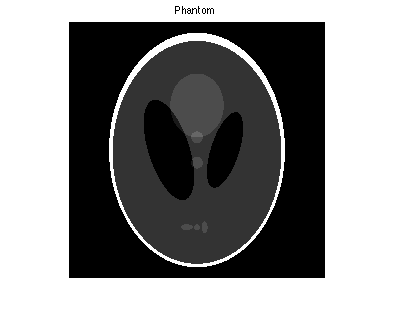
\includegraphics[width=\textwidth]{Images/phantom.png}
  \end{minipage}
  \hfill
  \begin{minipage}[b]{0.45\textwidth}
    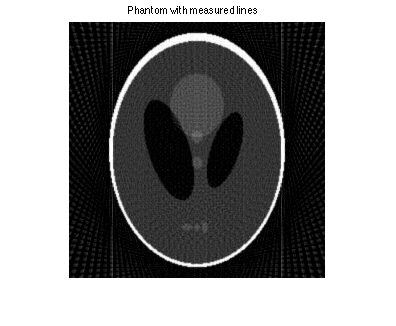
\includegraphics[width=\textwidth]{Images/phantom_measured.png}
  \end{minipage}
\end{figure}
\end{frame}

\begin{frame}{Sinogram}
\begin{figure}[!tbp]
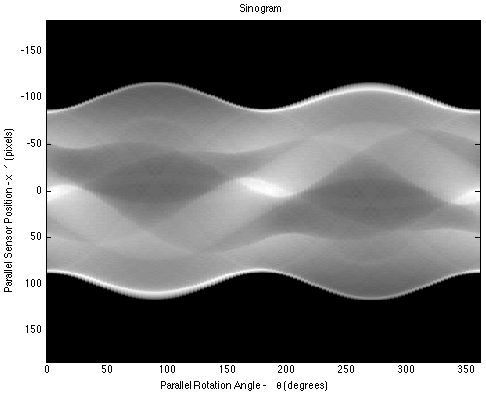
\includegraphics[width=0.9\textwidth]{../sinogram.png}
\end{figure}
\end{frame}

\begin{frame}{Solving inverse problems}
\begin{block}{First approach}
Minimizing the miss-fit against data:
$$
\min_{f} \mathcal{L}(\mathcal{R}(f),g)
$$
e.g. $\mathcal{L}(\mathcal{R}(f),g)=||\mathcal{R}(f)-g||_2^2$.
\end{block}

\textbf{Three classical techniques:}
\begin{itemize}
\item Pseudo-inverse of $\mathcal{T}$ using a mollifier.
\item Iterative regularization, starting with a fixed point iteration scheme for minimizing (iterative hard thresholding), and stop iterates before over-fitting.
\item Variational regularization, by introducing a functional $\mathcal{S}:X\longrightarrow \mathbb{R}$, that encodes a-priori information about $f_{\text{true}}$, e.g.\ sparsity under some dictionary.
$$
\min_{f\in X} [\mathcal{L}(\mathcal{T}f,g)+\lambda \mathcal{S}f] \quad \text{for fixed}\quad \lambda\geq 0
$$
$\lambda$ (regularization parameter) governs the influence of the a priori knowledge, choosing it is a problem.
\end{itemize}
\end{frame}

\begin{frame}{Learning comes into play}

One could ask to learn a pseudo-inverse $\mathcal{T}_{\Theta}(g)\approx f_{\text{true}}$ and learn the parameters $\Theta\in Z$ through a loss functional. 

\pause

\bigskip

Fully learned method are very dependent on the training set, one would like to combine a partially learned iterative method with known information of the problem (e.g.\ wavefront set).

\pause

\bigskip

\begin{itemize}
\item If $\mathcal{T}$ is local (e.g.\ deblurring problem) $\longrightarrow$ convolutional neural network and known pairs $(g,f_{\text{true}})$.
\item If $\mathcal{T}$ is global (e.g.\ Radon transform) $\longrightarrow$ CNN does not work, it becomes unfeasible to work with NN with fully connected layers.
\end{itemize}
\end{frame}

\begin{frame}{Alternative solutions}
\begin{enumerate}
\item Recast to image-to-image problem: perform some initial (non machine-learning) reconstruction (e.g.\ FBP), and then use standard CNN to denoise the initial reconstruction. Upside: it outperforms previous state of the art methods. Donwside: it does not give you more information than using just non-machine learning reconstruction.

\pause 

\item Incorporate enough a-priori information to make the problem tractable and learn the rest (Learned Primal-dual algorithm): First use CNN to update the data (dual step), then apply $\mathcal{T}^*$ and use the result as input to another neural network which updates the reconstruction (primal step), then apply $\mathcal{T}$ and use it as input to a neural network that updates the data, and so on. Upside: it separates the global aspect of the problem into the forward model and its adjoint and only need to learn local aspects. Downside: to train the NN one needs to perform back-propagation through this NN severak times. 
\end{enumerate}
\end{frame}

\begin{frame}{Wavefront set as extra information}
\begin{definition}[N-Wavefront set]
Let $N\in\mathbb{R}$ and $f$ a distribution on $\mathbb{R}^2$. We say $(x,\lambda)\mathbb{R}^2\times \mathbb{R}^2$ is a $N-$regular directed point if there exists a nbd.\ of $U_x$ of $x$, a smooth cutoff function $\Phi$ with $\Phi\equiv 1$ on $U_x$ and a nbd.\ $V_{\lambda}$ of $\lambda$ such that:
$$
(\Phi f)^{\wedge}(\eta)=O((1-|\eta|)^{-N}) \quad \text{for all}\quad \eta=(\eta_1,\eta_2) \quad \text{such that}\quad \frac{\eta_2}{\eta_1}\in V_{\lambda}
$$
The $N-$Wavefront set $WF^N(f)$ is the complement of the $N-$regular directed point. The Wavefront Set $WF(f)$ is defined as 

\begin{equation}
\label{eq:Wavefront-set}
WF(f)=\cup_{N>0}WF^N(f)
\end{equation}
\end{definition}
\textbf{Question?} How can one incorporate extra information from the $N-$Wavefront set of an image by knowing just its Radon Transform.
\end{frame}

\begin{frame}{Answer: Canonical shearlet transform of the sinogram}
\begin{block}{Classical Shearlet Transform}
$$
\langle f,\psi_{a,s,t}\rangle =\int_{\mathbb{R}^2}f(x)\overline{\psi_{a,s,t}(x)}dx
$$
where
$$
\mathcal{SH}(\psi)=\{\psi_{a,s,t}(x):=a^{-3/4}\psi (S_sA_ax-t):(a,s,t)\in \mathbb{R}_+\times\mathbb{R}\times\mathbb{R}^2\}
$$
and

$$
A_a:=
\left(
\begin{matrix}
a^1 & 0 \\
0 & a^{1/2}
\end{matrix}
\right)
\quad
S_s:=
\left(
\begin{matrix}
1 & s \\
0 & 1
\end{matrix}
\right)
$$
\end{block}
\end{frame}

\begin{frame}

\begin{theorem}[Resolution of the Wavefront set by continuous shearlet frames; Grohs, 2011] 
Let $\Psi$ be a Schwartz function with infinitely many vanishing moments in $x_2-$direction. Let $f$ be a tempered distribution and $\mathcal{D}=\mathcal{D}_1\cup\mathcal{D}_2$, where

 $\mathcal{D}_1$ =\{$(t_0,s_0)\in \mathbb{R}^2\times [-1,1]:$ for $(s,t)$ in a nbd.\ $U$ fo $(s_0,t_0)$, $|\mathcal{SH}_{\psi}f(a,s,t)|=O(a^k)$ for all $k\in\mathbb{N}$, with the implied constant uniform over $U$\} and

$\mathcal{D}_2$=\{ $(t_0,s_0)\in\mathbb{R}^2\times (1,\infty]:$ for $(1/s,t)$ in a nbd.\ $U$ of $(s_0,t_0)$, $|\mathcal{SH}_{\psi ^{\nu}}f(a,s,t)|=O(a^k)$ for all $k\in\mathcal{N}$, with the implied constant uniform over $U$\}. Then
$$
WF(f)^c=\mathcal{D}
$$
\end{theorem}

\pause

\begin{theorem}[O. \"Otkem et al., 2008]
Broadly speaking, a point on the $N-$Wavefront set of a distribution corresponds to a point on the $N+1/2-$Wavefront set of its Radon transform, with the corresponding directions.
\end{theorem}
\end{frame}

\begin{frame}{Only thing left: Shearlets on the sinogram}
\begin{itemize}
\item Using results of compactly supported shearlets and shearlets on bounded domains, one can construct a shearlet frame on the space of the sinogram $L^2_{x_1-2\pi}([0,2\pi)\times \mathbb{R})$, given by

$$
\psi_{a,s,t}^{x_1-2\pi}(x_1,x_2):=\sum_{\ell\in\{-1,0,1\}}\psi_{a,s,t}(x_1+2\pi\ell,x_2)
$$
where $\psi_{a,s,t}$ is a shearlet compactly supported on $[0,2\pi)\times \mathbb{R}$, whose corresponding system form a frame for $L^2([0,2\pi)\times \mathbb{R})$.

\pause

\item Then in the learned primal-dual algorithm one can incorporate as extra information the $N-$Wavefront set of the image by pulling back the $N+1/2-$Wavefront set captured by the proposed shearlet frame. This will let us to get a solution with minimum lost of the important features of the images.
\end{itemize}
\end{frame}

\begin{frame}{Thanks!}
\begin{center}
\Large{Questions?}
\end{center}
\end{frame}



\end{document}
